% !TEX root = ../../presentation.tex
% Meta: Workflow

\newlength{\height}\setlength{\height}{0.4cm}\relax

% Only for the header
\begin{slide}{Workflow}\end{slide}

\begin{slide}{Workflow: Programmiersprachen}
  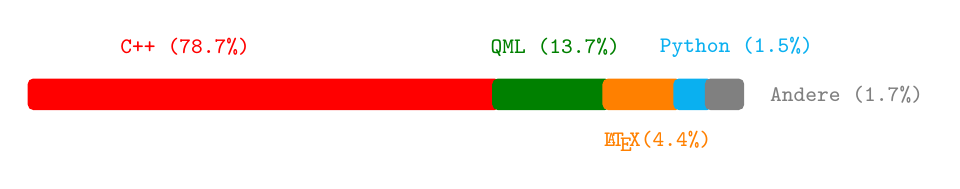
\begin{tikzpicture}
    % C++
    \fill [Red, rounded corners=2pt]
          (0, 0) rectangle ++(6, \height);
    \draw [Red] (2, {\height + 0.4cm})
          node {\footnotesize\texttt{C++ (78.7\%)}};

    % QML
    \fill [Green, rounded corners=2pt]
          (5.9, 0) rectangle ++(1.5, \height);
    \draw [Green] (6.7, {\height + 0.4cm})
          node {\footnotesize\texttt{QML (13.7\%)}};

    % LaTeX
    \fill [orange, rounded corners=2pt]
          (7.3, 0) rectangle ++(1, \height);
    \draw [orange] (8, -0.4cm)
          node {\footnotesize\texttt{\LaTeX (4.4\%)}};

    % % Python
    \fill [ProcessBlue, rounded corners=2pt]
          (8.2, 0) rectangle ++(0.5, \height);
    \draw [ProcessBlue] (9, {\height + 0.4cm})
          node {\footnotesize\texttt{Python (1.5\%)}};

    % % Other
    \fill [Gray, rounded corners=2pt]
          (8.6, 0) rectangle ++(0.5, \height);
    \draw [Gray] (10.4, {\height/2})
          node {\footnotesize\texttt{Andere (1.7\%)}};
  \end{tikzpicture}
\end{slide}

\begin{slide}{Workflow: Programmiersprachen}
  \small
  \begin{tabular}{lrrr}
    \textbf{Programmiersprache} & \textbf{Kommentarzeilen} & \textbf{Codezeilen} & \textbf{Gesamt} \\
    \midrule
    C\texttt{++} & 17475 & 23637 & 41112 \\
    QML & 1973 & 5567 & 7540 \\
    TeX & 247 & 3966 & 4213 \\
    Python & 242 & 543 & 785 \\
    JSON & 0 & 531 & 531 \\
    SASS & 11 & 439 & 450 \\
    CMake & 117 & 308 & 425 \\
    Markdown & 0 & 82 & 82 \\
    JavaScript & 27 & 71 & 98 \\
    \bottomrule
    Alle & 20092 & 35144 & 55236
  \end{tabular}
\end{slide}

\begin{slide}{Workflow: Methoden \& Hilfsmittel}
  \onslide<2->{
    {\Large \emph{Definitions of Done}}
    \vspace{0.25cm}
  }

  \small
  \begin{enumerate}
    \item<3-> Code wurde geschrieben,
    \item<4-> Unit Tests stehen und passen (\textbf{GoogleTest, Travis}),
    \item<5-> Der Code ist dokumentiert (\textbf{Doxygen}),
    \item<6-> Der Code ist formattiert (\textbf{clang-format}),
    \item<7-> Ein Pull Request wurde ge\"{o}ffnet (\textbf{Waffle, GitHub}),
    \item<8-> OK von Code-Reviewern (\textbf{GitHub}),
    \item<9-> Merge des Feature Branch in den Master Branch (\textbf{Git}),
    \item<10-> Profit.
  \end{enumerate}
\end{slide}
